\documentclass[12pt]{article}
%\pdfoutput=1
\usepackage[utf8]{inputenc}
\usepackage[section]{placeins}
\usepackage{amsmath}
\usepackage{amsfonts}
\usepackage{amssymb}
\usepackage{graphicx}
%\usepackage[executivepaper,margin=0.5in]{geometry}
\usepackage[space]{grffile}
\usepackage{flafter}
\usepackage[backend=biber, giveninits=true]{biblatex}
\usepackage{multirow}
\usepackage{tikz}
\usetikzlibrary{shapes,arrows}
\usepackage{epsfig,amsfonts,amsthm}
\usepackage[normalem]{ulem}
\usepackage{amsmath,amssymb}
\usepackage{array}
\usepackage{amsmath}
\usepackage{amsfonts}
\usepackage{amssymb}
\usepackage{subfig}
\usepackage{wrapfig}
\usepackage{graphicx}
\usepackage{xcolor}
\usepackage[normalem]{ulem}


\newcommand{\be}{\begin{equation}}
\newcommand{\ee}{\end{equation}}
\newcommand{\bea}{\begin{eqnarray}}
\newcommand{\eea}{\end{eqnarray}}
\newcommand{\dst}{\displaystyle}
\newcommand{\fr}[2]{\frac{{\dst #1}}{{\dst #2}}}
\newcommand{\f}{\phi}
\newcommand{\fd}{\phi^\dagger}
\renewcommand{\Re}{\mathrm{Re }}
\renewcommand{\Im}{\mathrm{Im }}
\newcommand{\doublet}[2]{ \left( \begin{array}{c}#1 \\ #2 \end{array}\right) }
\newcommand{\bracket}[2]{ \langle #1|#2 \rangle}
\newcommand{\lr}[1]{ \langle #1 \rangle}
\newcommand{\Tr}{\mathrm{Tr}}
\newcommand{\Z}{\mathbb{Z}}
\newcommand{\triplet}[3]{ \left( \begin{array}{c}#1 \\ #2 \\ #3 \end{array}\right) }
\usepackage{color}

\providecommand{\calV}{\mathcal{V}}
\providecommand{\RR}{{\mathbb{R}}}
\providecommand{\vr}{\vec{r}}

\def\lsim{\mathrel{\rlap{\lower4pt\hbox{\hskip1pt$\sim$}}
    \raise1pt\hbox{$<$}}}         %less than or approx. symbol
\def\gsim{\mathrel{\rlap{\lower4pt\hbox{\hskip1pt$\sim$}}
    \raise1pt\hbox{$>$}}}         %greater than or approx. symbol




\newcommand{\CenterObject}[1]{\vcenter{\hbox{#1}}}
\newcommand{\CenterEps}[2][1]{\ensuremath{\vcenter{\hbox{\includegraphics[scale=#1]{#2.eps}}}}}
\newcommand{\SuperField}[1]{\hat{#1}}

\def\D{\mathrm{d}}
\def\I{\mathrm{i}}
\def\SU{\,\text{SU}}
\def\SO{\,\text{SO}}
\def\U{\,\text{U}}
\def\O{\,\text{O}}
\def\SL{\,\text{SL}}
\def\beq{\begin{equation}}
\def\eeq{\end{equation}}
\def\bea{\begin{eqnarray}}
\def\eea{\end{eqnarray}}

\def\eps{\epsilon}
\def\epsb{\bar{\epsilon}}
\def\epstensor{\varepsilon}


\def\Fla{\theta}
\def\Flb{\bar{\theta}}


\def\Pauli{\tau}
\def\<{\left\langle}
\def\>{\right\rangle}
\def\ChargeC{\mathrm{C}}
\def\chargec{\mathrm{C}}

\newcommand{\ChargeConjugate}[1]{{#1}^\ChargeC}

\newcommand{\GeV}{{\ensuremath\rm \,GeV}}

\def\DS{\color{red}}

\usepackage[normalem]{ulem}



\providecommand{\calV}{\mathcal{V}}
\providecommand{\RR}{{\mathbb{R}}}
\providecommand{\vr}{\vec{r}}

\def\lsim{\mathrel{\rlap{\lower4pt\hbox{\hskip1pt$\sim$}}
    \raise1pt\hbox{$<$}}}         %less than or approx. symbol
\def\gsim{\mathrel{\rlap{\lower4pt\hbox{\hskip1pt$\sim$}}
    \raise1pt\hbox{$>$}}}         %greater than or approx. symbol



\def\D{\mathrm{d}}
\def\I{\mathrm{i}}
\def\SU{\,\text{SU}}
\def\SO{\,\text{SO}}
\def\U{\,\text{U}}
\def\O{\,\text{O}}
\def\SL{\,\text{SL}}
\def\beq{\begin{equation}}
\def\eeq{\end{equation}}
\def\bea{\begin{eqnarray}}
\def\eea{\end{eqnarray}}
\def\eps{\epsilon}
\def\epsb{\bar{\epsilon}}
\def\epstensor{\varepsilon}
\def\Fla{\theta}
\def\Flb{\bar{\theta}}
\def\Pauli{\tau}
\def\<{\left\langle}
\def\>{\right\rangle}
\def\ChargeC{\mathrm{C}}
\def\chargec{\mathrm{C}}
\newcommand{\gev}{\mathrm{\,GeV}}
\newcommand{\bt}{\begin{tabular}}
\newcommand{\et}{\end{tabular}}
\newcommand{\un}{\underline}
\newcommand{\ov}{\overline}
\newcommand{\ds}{\displaystyle}
\newcommand{\rre}{\mathrm{Re}}
\newcommand{\iim}{\mathrm{Im}}

\usepackage{hyperref}

\hypersetup{
   colorlinks=true,       % false: boxed links; true: colored links
   linkcolor=blue,        % color of internal links
   citecolor=red,         % color of links to bibliography
   filecolor=magenta,      % color of file links
   urlcolor=cyan,           % color of external links
   linktocpage = true,
   }

\usepackage{tikz}
\usetikzlibrary{decorations.pathmorphing,decorations.markings}


\usepackage{graphicx}%Täl saa laitettuu kuvii. Esim. ps filei. Kun haluu laittaa .epsi tai .eps tiedostoja, niin laittaa eka \includegraphics{nimi.eps}. Sit kääntää pdflatex:lla ja kuva tulee.



%Määritellään nyt milä tyylillä feynmanin graafit piirtyy.
\tikzset{
photon/.style={decorate, decoration={snake,amplitude=2pt, segment length=5pt}, draw=black},
particle/.style={draw=black, postaction={decorate}, decoration={markings,mark=at position .5 with {\arrow[draw=black]{>}}}},
antiparticle/.style={draw=black, postaction={decorate}, decoration={markings,mark=at position .5 with {\arrowreversed[draw=black]{>}}}},
gluon/.style={decorate, draw=black, decoration={coil,amplitude=4pt, segment length=5pt}},
goldstone/.style={draw=green,postaction={decorate},decoration={markings,mark=at position .5 with {\arrow[draw=blue]{>}}}}
}

\let\vec\mathbf
% if we created names here we can quickly change capitalisation etc.
% varient of delta R
\newcommand{\stoppingdeltar}{\ensuremath{R}}
\newcommand{\ktstoppingdeltar}{\ensuremath{R_{k_T}}}
\newcommand{\distancedeltar}{\ensuremath{\Delta R}}
%b related things, so that we always get the math-mode right
\newcommand{\beau}{\ensuremath{b}}
\newcommand{\bbar}{\ensuremath{\bar{b}}}
\newcommand{\bthing}[1]{\ensuremath{b\text{-#1}}}
% some names for consistent capitalisation
\newcommand{\genkt}{generalised $k_T$}
\def\antikt{anti-$k_T$}
\newcommand{\itercone}{iterative cone}
\newcommand{\spectral}{spectral}
\def\fastjet{{\tt FASTJET}}

\bibliography{writeup}   
\graphicspath{{./graphics/}}


%%%%%%%%%%%%%%%%%%%%%%%%%%%%%%%%%%%%%%%%%%%%%%%%%%%%%%%%%%%%%%%%%%%%%%%%
%%BEGINNING OF TEXT
%%%%%%%%%%%%%%%%%%%%%%%%%%%%%%%%%%%%%%%%%%%%%%%%%%%%%%%%%%%%%%%%%%%%%%%%
\allowdisplaybreaks[2]
\addtolength\textwidth{2cm}
\evensidemargin 0cm
\oddsidemargin  0cm
%\sloppy
\begin{document}
%\bibliographystyle{OurBibTeX}


\title{\hfill ~\\[-50mm]
                  \textbf{Spectral Clustering for Jet Physics
                }        }
%\date{}

\author{\\[-5mm]
S. Dasmahapatra\footnote{E-mail: {\tt sd@ecs.soton.ac.uk}} $^{1}$,\
H.A. Day-Hall\footnote{E-mail: {\tt hadh1g17@soton.ac.uk}} $^{2,3}$,\
B. Ford\footnote{E-mail: {\tt b.ford@soton.ac.uk}} $^{2}$,\ \\
S. Moretti\footnote{E-mail: {\tt stefano@phys.soton.ac.uk}} $^{2,3}$,\
C.H. Shepherd-Themistocleous\footnote{E-mail: {\tt claire.shepherd@stfc.ac.uk}} $^{3}$
\\ \\
\emph{\small $^1$School of Electronics and Computer Science, University of Southampton,}\\
\emph{\small Southampton, SO17 1BJ, United Kingdom}\\
\emph{\small $^2$School of Physics and Astronomy, University of Southampton,}\\
\emph{\small Southampton, SO17 1BJ, United Kingdom}\\
\emph{\small  $^3$Particle Physics Department, Rutherford Appleton Laboratory,}\\
\emph{\small Chilton, Didcot, Oxon OX11 0QX, United Kingdom}\\[4mm]
 }
%
\maketitle
%
\vspace*{-10mm}
%
\begin{abstract}
\noindent
{{\color{magenta} We present a new method of jet definition as an alternative to the clustering methods, such as \antikt, that are based directly on kinematic data by, instead, using kinematic relations to define a spectral representation of the particles.} 
 The performance of this algorithm in analysing  
\(gg\to H_{125\,\text{GeV}} \rightarrow H_{40\,\text{GeV}} H_{40\,\text{GeV}} \rightarrow b \bar{b} b \bar{b}\),
\(gg\to H_{500\,\text{GeV}} \rightarrow H_{125\,\text{GeV}} H_{125\,\text{GeV}} \rightarrow b \bar{b} b \bar{b}\)
and
\(gg,q\bar q\to t\bar t\to b\bar b W^+W^-\to b\bar b jj \ell\nu_\ell\) events from 
 Monte Carlo (MC) samples {\color{magenta} in reconstructing the relevant final states} is compared to that of the \antikt algorithm.
 Measures of infra-red (IR) safety, both soft and collinear, are also studied. {\color{magenta} We find that the ability of spectral clustering in reconstructing mass peaks is comparable to that of \antikt under realistic acceptance and selection criteria.  Unlike the standard approach in which the jet cone size needs to be adapted to the  kinematics of the events under study, the new algorithm does not require an adjustment of its parameter settings for the processes analysed.}}
 \end{abstract}
\thispagestyle{empty}
\vfill
\newpage
%
    \section{Jet Clustering}\label{sec:JetClustering}
This next section considers a completely novel approach to jet clustering, spectral clustering.

As mentioned previously, the default choice for jet clustering tends to be one of there algorithms;
the anti-kt algorithm~\cite{Cacciari2008akt}, the Cambridge-Aachen algorithm~\cite{Wobisch1998caJet} and the kt algorithm~\cite{Ellis1993ktJet}.
They have been the default choice for some time because they have a number of desirable properties.
They are infrared safe, excellent implementations of them are available (see \fastjet{}~\cite{Cacciari2011FastJet})
and it is flexible enough to capture many signals with minimal parameter change.
These algorithms are recursive and agglomerative.
A recursive algorithm is well suited to clustering objects when the number of groups is not known at outset.
Agglomerative algorithms are easier to design in a manner that is infrared safe,
as they can recombine soft and collinear emissions in early steps.

Finding a clustering method that compares favourably to these algorithms is challenging.
Spectral clustering is a candidate that has had considerable success in other studies.
In fluid dynamics spectral clustering has been used to identify the motion
of vortices~\cite{hadjighasem2016votex}, finding that it is possible
to successfully identify the vortex structures in cases with less data available.
It was also seen that spectral clustering was proficient at determining the correct number
of clusters to be found in the fluid.
To reduce the risk of blackouts, power grids may be subdivided into `islands'.
The ideal allocation is found by minimising power flow between islands,
and it was shown in~\cite{fennelly2014power} that spectral clustering
can produce a good solution in less time than other algorithms commonly used for this problem.

%Adaptive spectral clustering with application to tripeptide conformation analysis~\cite{haack2013AdaptiveSC}.  %TODO

To the authors knowledge this clustering algorithm has not yet been applied to jet physics, %TODO - double check.
however, given its recursive, agglomerative form it could be a good fit.

    \FloatBarrier
    \section{Theory of spectral clustering}\label{sec:spectral_theory}

Collimated emissions of particles are clustered by jet algorithms.  A
representation of observable particles that preserves and accentuates local information
motivates the Laplacian eigenmap~\cite{BelkinNiyogi2003} and spectral
clustering~\cite{NgJordanWeiss2002}.
Spectral clustering is a method by which a set of points are represented in a new space,
called the embedding space, in which they can be easily clustered.  Coordinates of the
points in the embedding space are expressed in terms of the eigenvectors and eigenvalues
of an associated Laplacian matrix, hence the name.

The particles in an event are described first as nodes of a graph and
edges capturing a notion of similarity between them.
The theory behind the
construction of the embedding space is a relaxation of criteria that would precisely
partition nodes into separate disconnected subgraphs.
An excellent description can be found in~\cite{luxburg2007spectraltutorial}; a short
summary is given here.

At the start we have a group of points with coordinates, which should be split into a  number \(c\) of predetermined clusters.
Applying the spectral clustering method requires making these points into a graph.
A simple way to do this would be to consider the points to be the nodes of a fully connected graph.
The vertex of the graph joining node (or point) \(i\) and \(j\) has weight \(a_{i, j}\),
which should grow with the probability of \(i\) and \(j\) being in the same group.

The initial aim is to identify which of the components each point belongs to,
by sorting the graph into subgraphs, \(G_k\), where \(k=1 \dots c\).
Minimising the NCut objective is a function that captures this aim, where 
\begin{equation}
    \text{NCut} = \frac{1}{2}\sum_k\frac{W(G_k, \bar{G_k})}{\text{vol}(G_k)},
\end{equation}\label{eqn:cost_function}
where \(W(G_k, \bar{G_k})\) is the sum of all the vertex weights that must be dropped
to separate the cluster \(G_k\) from the rest of the graph, \(\bar{G_k}\).
So that \( W(G_k, \bar{G_k}) = \sum_{i \in G_k, j \in \bar{G_k}} a_{i, j} \).
In the denominator \(\text{vol}(G_k) = \sum_{i \in G_k} \sum_{j} a_{i, j}\),
the sum of all affinities connecting to a point in \(G_k\).
This denominator is used to penalise forming small clusters.

In order to determine which point will go in which \(G_k\), a set of indicator vectors must be found.
Membership of cluster \(G_k\) will be recorded in the indicator vector \(h_k\):
\begin{equation}\label{eqn:indicator}
    h_{i, k}= 
    \begin{cases}
        1/\sqrt{\text{vol}(G_k)}& \text{if point } i \in G_k ,\\
        0             & \text{otherwise},
    \end{cases}
    .
\end{equation}

To find these indicator vectors the graph is represented by the graph Laplacian, \(L\), a square
matrix with as many rows and columns as there are points.
To construct this Laplacien we define two other matrices;
an off diagonal matrix 
\(A_{i, j} = (1 - \delta_{i, j})a_{i, j}\)
and a diagonal matrix
\(D_{i, j} = \delta_{i, j}\sum_q a_{i, q}\).
Then the symmetric Laplacian can be simply written as;
\begin{equation}\label{eqn:symmetric_laplacian}
    L = D^{-\frac{1}{2}} (D - A) D^{-\frac{1}{2}}
\end{equation}

Notice that this is a real symmetric matrix
and, therefore all its eigenvalues are real.
Considering just one cluster, \(G_k\), when the Laplacian is multiplied by its indicator vector,
the result is the term that NCut seeks to minimise for that cluster.
\begin{equation}
    h_k'Lh_k = \frac{1}{\text{vol}(G_k)}\sum_{i \in G_k, j \in G_k} \left(\delta_{i, j}\sum_{l} a_{l, i} - a_{i, j} \right) = \frac{W(G_k, \bar{G_k})}{\text{vol}(G_k)}
\end{equation}
To obtain the sum of all the terms, stack the indicator vectors into a matrix,
\( h'_k L h_k = (H'L H)_{kk}\),
and the NCut aim described earlier becomes the trace,
\begin{equation} \text{NCut}(G_1,G_2, \dots G_n) \equiv \frac{1}{2} \sum_{k=1}^n \frac{W(G_k, \bar{G_k})}{\text{vol}(G_k)} = \text{Tr}(H'LH),\end{equation}
where \(H'H = I\).
This is still an NP hard problem, however if we relax the requirements made on \(h\) in Eqn.~\ref{eqn:indicator},
allowing the elements of \(h\) to take arbitrary values, then the Rayleigh-Ritz theorem provides a solution.
Trace minimisation in this form is done
by finding the eigenvectors of \(L\) with smallest 
eigenvalues.
Due to the form of the Laplacian, there will be an eigenvector with components all of the same value and its eigenvalue will be \(0\).
This corresponds to the trivial solution of considering all points to be in one group.
The next \(c\) eigenvectors of \(L\), sorted by smallest eigenvector, are the indicator vectors needed to allocate points to \(c\) clusters.

These indicator vectors are then used to determine position of the points in the embedding space.
Each indicator vector has as many elements as there are points to be clustered,
so the coordinates of a point are the corresponding elements or the indicator vectors.
This is all the information the theory of spectral clustering provides.
The steps required to make use of this information are not dictated by the theory,
and they must be carefully selected to respect the physics.

Using the positions in embedding space the points can be gathered agglomeratively,
so that we do not need to chose a predetermined number of clusters.

\subsection{Distance in the embedding space}\label{sec:embedding_distance}
When the relaxed spectral clustering algorithm is used to create an embedding space, points in a group will not be at exactly the same coordinates.
Each point can be seen as a vector, the direction of this vector indicates the group to which this point should be assigned.
The magnitude indicates the confidence with which the assignment is made.
Changes in magnitude cause the Euclidean distance between the corresponding points to grow.
An angular distance is appropriate, though. 
The angular distance will grow when the eigenvectors indicating the point have less overlap
and this is what should be measured.

\subsection{Information in the eigenvalues}\label{sec:eig_norm}
When the clusters in the data are very clear, the situation is closer to the ideal one and the eigenvalues will be closer to \(0\).
The smaller an eigenvalue is, the more like a perfect indicator vector the corresponding eigenvector is.
It is possible to make use of this information.

In a traditional application of spectral clustering, the number of clusters desired, \(c\), is predetermined.
The embedding space is created by taking \(c\) eigenvectors with smallest eigenvalues, excluding the trivial eigenvector.
The embedding space then has \(c\) dimensions.
This follows from a relaxation of the concept of indicator vectors.

When forming jets we do not know from the outset how many clusters to expect in the dataset,
so the number of eigenvectors to keep is not clear.
While we could chose a fixed, arbitrary number of eigenvectors, this is suboptimal.
A better approach is to take all non-trivial eigenvectors corresponding to eigenvalues
smaller than some limiting number, \(\lambda_\text{limit}\).
For a symmetric matrix the eigenvalues will be \(0 < \lambda < 2\),
so \(\lambda_\text{limit} = 0.5\) would be a reasonable choice.
Then, the number of dimensions in the embedding space will vary,
according to the number of non-trivial eigenvectors with corresponding \(\lambda < \lambda_\text{limit}\).

There is one more manipulation from the information in the eigenvalues.
The dimensions of this embedding space are not of equal importance,
those with higher eigenvalues being less interesting.
This can be accounted for by dividing the eigenvector by some power, \(\beta\), of the eigenvalue.

Let the eigenvectors for which \(\lambda < \lambda_\text{limit}\) be
\begin{equation}
    L_{i, j} (h_n)_j = \lambda_n (h_n)_i.
\end{equation}
Then, the coordinates of the \(j^\text{th}\) point in the \(c\) dimensional embedding space
become \(m_j = \left(\lambda_1^{-\beta} (h_1)_j, \dots \lambda_c^{-\beta} (h_c)_j,\right)\).
In effect the \(n^\text{th}\) dimension is compressed by a factor \(\lambda_n^\beta\),
so the larger \(\lambda_n\) the greater the compression.

\subsection{Stopping conditions}\label{sec:stopping_condintion}

If a recursive algorithm is to be chosen, like in the \genkt{} algorithm, a stopping condition is needed.
A stopping condition based on smallest distance between points in the embedding space does not prove to be stable,
as the distribution  in the number of dimensions in the embedding space changes sharply from event to event.

The average distance between points is more stable.
If this were used in physical space it would force roughly the same number of clusters to form each time,
however, the variable number of dimensions in the embedding space is now an advantage.
The  clearer information found about clusters in the points the more dimensions the embedding space will contain,
as described in section~\ref{sec:eig_norm}.

Say, the data contains two points that would form a good cluster.
If those two points are combined into one, that cluster is complete,
fewer clusters remain unfinished
and the information for clustering the resulting points will be reduced.
When the embedding space is recalculated for the new points, it will likely have fewer dimensions.
In a space with fewer dimensions the mean distance between the points naturally falls.
Thus, the mean distance in the embedding space is a good indicator of the number of unfinished clusters available.
In short, the mean distance in the embedding space makes a natural cut-off.

    \FloatBarrier
    \subsection{Method}
\subsubsection{Particle data}
The dataset used for the majority of this work is a simulated Higgs cascade decay.
One Standard Model (SM) Higgs at \(125\)GeV decays to two light Higgs at \(40\)GeV,
which in turn decay to \beau{}-\bbar{} quark pairs.
That is \(H_{125\text{GeV}} \rightarrow h_{40\text{GeV}} h_{40\text{GeV}} \rightarrow \beau \bbar \beau \bbar\).


This dataset has the desirable property of creating \bthing{jets} with a range of geometries
owing to the boost provided by large mass of the SM Higgs and
the high chance of overlap with 4 \bthing{quarks} in the event.
Other radiation from the protons is also included.  % TODO clarify exactly what background is in here!


Before any evaluation can be performed on the final state of the simulation
particles that ended outside the range of the silicon tracker (\(|\eta|>2.5\))
or particles with low transverse momentum (\(p_T < 0.5\) GeV) are cut.
This is to mimic restrictions from reconstruction accuracy.

\begin{figure}[htp]
    \begin{minipage}[c]{0.5\textwidth}
        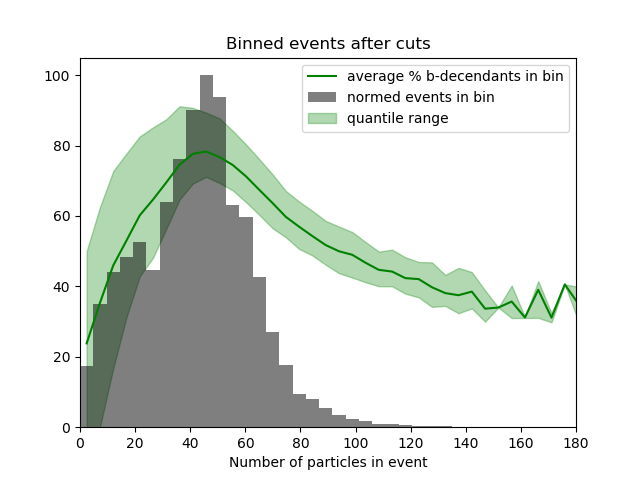
\includegraphics[width=1\textwidth]{graphics/binned_events.png}
    \end{minipage}\hfill
    \begin{minipage}[c]{0.45\textwidth}
        \caption{The end state particle in the simulated events are filtered
            with the standard cuts, \(p_T > 0.5\), \(|\eta| < 2.5\).
            The events are binned according to how many particles remain after the cuts.
            The percentage of \bthing{descendants} in the remaining event after the cuts
            is averaged for each bin and plotted on the same axis.
            After the cuts have been applied most events are left with around \(50\) particles.
                 The percentage of particles that are descendant from a \bthing{quark} varies,
                 it is at it's highest in events with \(50\) particles,
             and most variable in events will small multiplicity.}\label{fig:bdecendantpercent}
    \end{minipage}
\end{figure}    

A particle is considered a \bthing{descendant} if is found in the chain of decays from a \bthing{quark}.
After cuts, \(72\%\) of events have at least \(5\) \bthing{descendants} and \(5\) non \bthing{descendants} available.
Exactly how the percentage of \bthing{descendants} changes with event size is visualised in figure~\ref{fig:bdecendantpercent}.

\subsubsection{Clustering algorithm}\label{sec:spectralmethodalgo}
Now the implementation of the theory described in section~\ref{sec:spectral_theory} will be specified.
For every simulated event this process if used to select a clustering.

\begin{enumerate}
    \item \label{step:start} The particles are to be used to form the nodes of a graph,
    the edges of which will be weighted by some measure of proximity between the particles known as affinity.
    To obtain an affinity, first a distance is obtained; \(d_{i,j} = \sqrt{(y_i - y_j)^2 + (\phi_i - \phi_j)^2}\)
    where \(y_i\) is the rapidity of particle \(i\) and \(\phi_i\) is the barrel angle is particle \(i\).

    \item The distance shrinks as particles become similar, to obtain an affinity this must be transformed so that
    the value grows with increasing similarity.
    This is done by taking an inverse so that \(a_{i,j} = 1/d_{i,j}\), as done in~\cite{hadjighasem2016votex}. % TODO check you stick with this

    \item These affinities allow the construction of a Laplacien.
    The Laplacien used is the unnormalised Laplacien, which has \(\sum_j a_{i,j}\) in the \(i\)th
    diagonal entry (also known as the degree of node \(i\)) and \(-a_{i,j}\) of the diagonal 
    in column \(i\) row \(j\).

    \item From the Laplacien a predetermined number of eigenvectors are calculated to create the embedding space.
    The eigenvectors have as many elements as there are particles, and the coordinates of
    the \(i\)th particle in the embedding space is the \(i\)th element of each eigenvector.

    \item The first clustering can be done based on 
    a measure of distance derived from the particles \(p_T\) and it's position in the embedding space.
    The \(p_T\) is used as in the Luclus~\cite{moretti1998new}, with a variable exponent, \(q\);
    \[p_T \text{ factor} = \left(\frac{{p_T}_i{p_T}_j}{s({p_T}_i+{p_T}_j)}\right)^q\].
    Where \(s\) is the invariant mass of all observed particles in the event, it is used
    to make the \(p_T\) factor unitless.
    The embedded distance is euclidean distance in the embedding space multiplied by this factor.

    \item The two object that have the smallest embedding distance are combined.
    In physical space the combined object is created by summing the respective four momenta,
    in the embedding space two methods for locating the combined object are tried.
    \begin{enumerate}
        \item In a \spectralmeanjet{} clustering the location of the combined object is the
        geometric mean of the inputs. The clustering then continues to combine things in this manner.
        \item In a \spectralfulljet{} once two object have been combined in physical space
            the embedding space is recalculate from step~\ref{step:start}. 
    \end{enumerate}

    \item When the closest object to a particle in the embedding space is further away than \stoppingdeltar{}
    then the combined object is considered to be a complete jet and removed from future clustering.
\end{enumerate}
To provide a basis for comparison the results of clustering with an anti-kt algorithm (as in~\cite{Cacciari2008akt}) is also shown.


    \FloatBarrier
    \section{Results}

Before the behaviour of the algorithms is analysed, some plots of kinematic variables are shown
in Fig.~\ref{fig:kinematics}.
It can be seen that the algorithms do not greatly differ on the kinematics of the events.
In particular, \spectral{} clustering does not appear to sculpt any distributions in any of the datasets involving Higgs bosons and top (anti)quarks.


\begin{figure}[htp]
%    \begin{minipage}[c]{0.7\textwidth}
    \begin{center}
    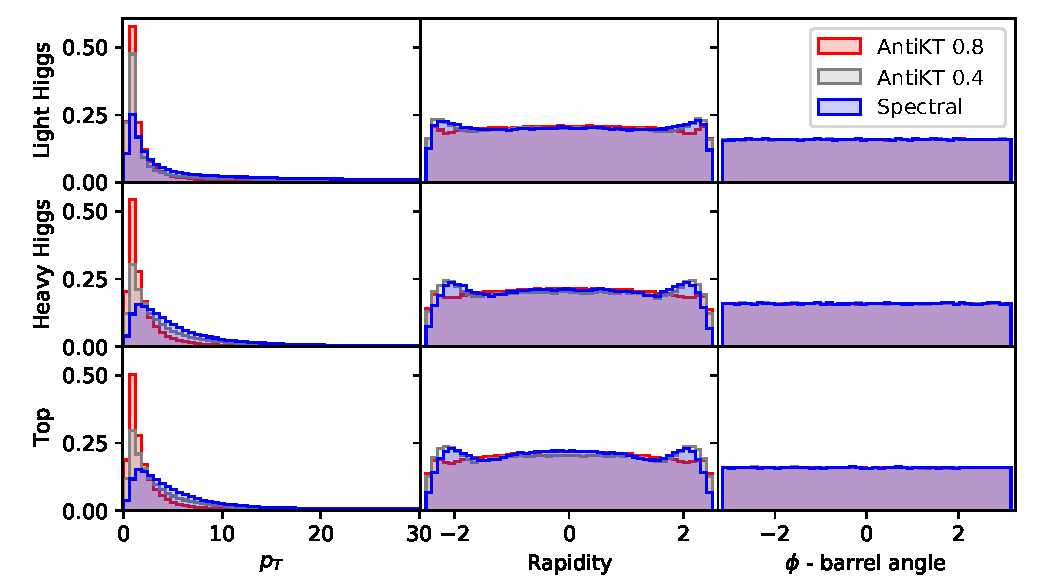
\includegraphics[width=\textwidth]{graphics/kinematics}
%\end{minipage}
    %\begin{minipage}[c]{0.25\textwidth}
        \caption{Basic jet variables for each of the analysis datasets and three clustering algorithms.
            In the first column there is some noticeable differences in the transverse momentum.
            In the second column the rapidity shows that
            the algorithms cluster jets at the edge of the barrel slightly differently.
            In the third column the barrel angle show no noticeable changes.
        }\label{fig:kinematics}
%\end{minipage}
\end{center}
\end{figure}

\subsection{IR safety}
Shape variables (see the QCD section of Ref.~\cite{Altarelli:116932} for a useful review), such as jet mass, thrust, sphericity and oblataness,  are sensitive to IR divergences.
For each configuration of the clustering algorithm we expect an IR safe algorithm to present a stable transition
in a shape variable from the LO to NLO datasets, as significant
changes in the spectra would indicate sensitivity to soft and collinear radiation.
The clustering and evaluation here is done using the \underbar{3-jets} dataset, as described in Sec.~\ref{sec:particle_data}.
Shape variables are calculated from the total momentum of the 4 jets with highest \(p_T\) in each event.
This comparison is made in Fig.~\ref{fig:IRC_singles2}.
It can be seen in this figure that little difference exists between \genkt{} and \spectral{} clustering, so as to reinforce that they are both IR safe.
{\textcolor{red}{What data set has been used here? Also, it would be woth to discuss why the distributions are so different for the case of the Mass variable. Finally, is the latter just the invariant mass formed by all tracks/particles in each jet?}\textcolor{blue}{H. I have now specifed the dataset and the choice of momentum vectors in each event. I also changed the parameters of genkt/spectral used so that they minimc each other. It just wanted a diferent parameter choice.}}

\begin{figure}[htp]
    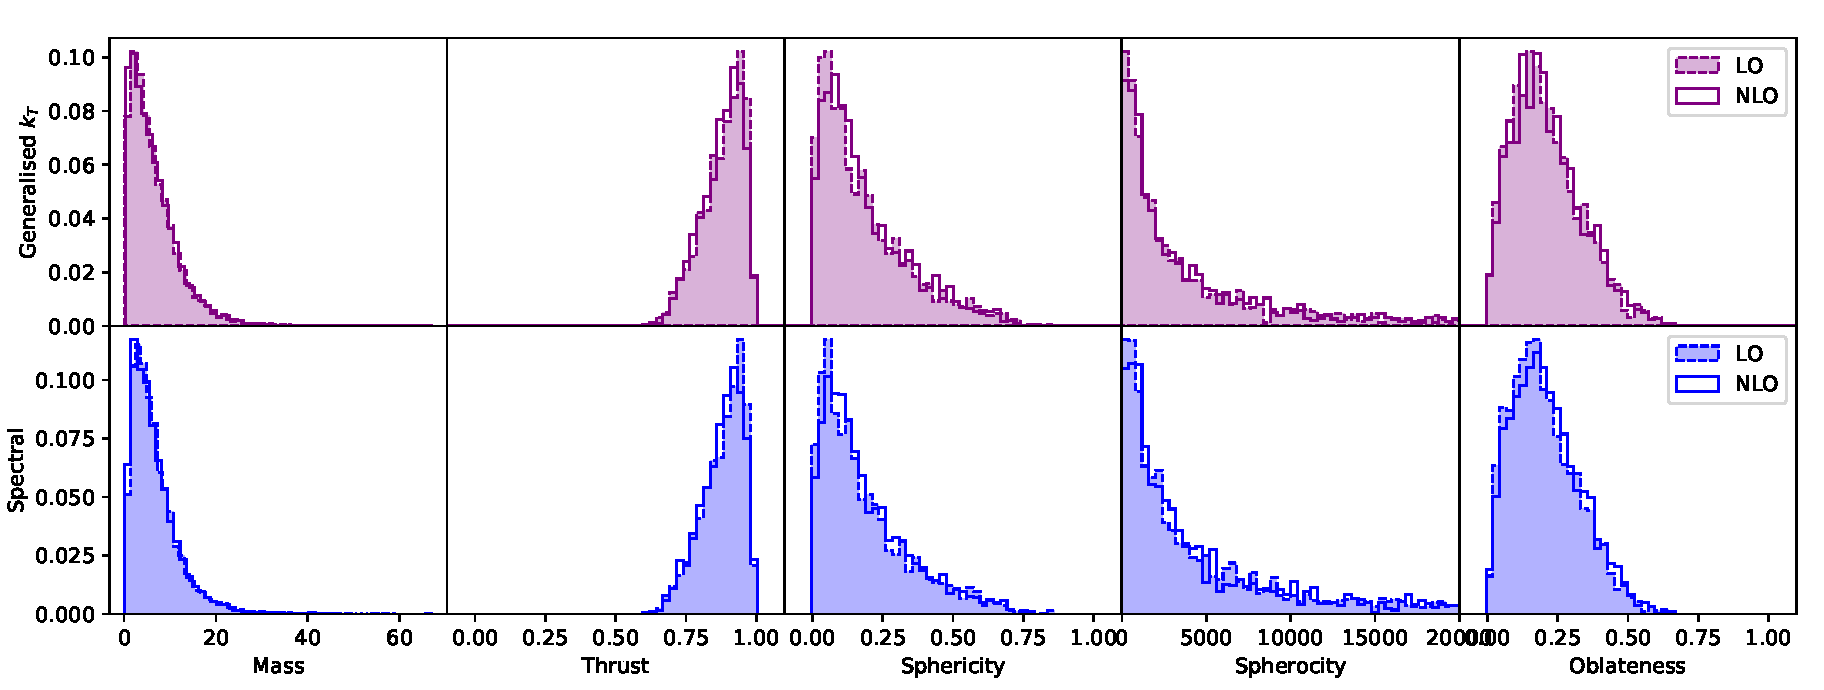
\includegraphics[width=\textwidth]{graphics/array_of_variables2_filled}
    \caption{Spectra for jet properties created with LO and NLO datasets.
             The \(4\) jets with highest \(p_T\) from each event are used in aggregate as an average to 
             form these plots.
             The columns from left to right are: the jet mass, 
             thrust, sphericity and oblateness.
             Algorithms where configured (i.e., settings of \stoppingdeltar{})
             to give sensible results on
             this dataset, therefore distributions may not represent worst case scenarios.
             %Looking at these graphs it is not immediately clear that the \genkt{}
             %algorithm is IR safe and the Iterative Cone algorithm is unsafe, 
         %much less what the status of Spectral clustering is.
         }\label{fig:IRC_singles2}
%    \begin{minipage}[c]{0.47\textwidth}
%        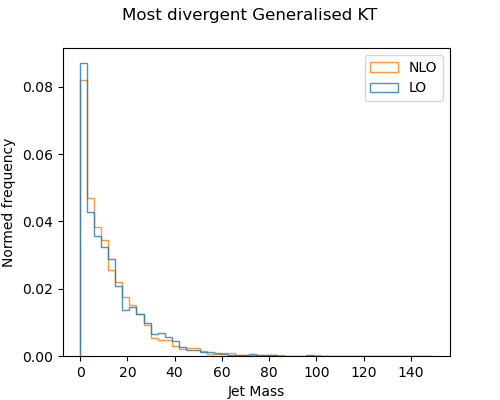
\includegraphics[width=\textwidth]{graphics/worst_antikt_histOnly.png}
         %        \caption{The jet mass spectra of the \genkt{} algorithms that
%                 differed the most between LO and NLO datasets.
%                 This algorithm had a \(p_T\) exponent of \(1.\),
%                 (so the form of the \(p_T\) factor is between Cambridge-Aachen and KT),
%                 it used taxi-cab distances in physical space
%                 and \(\stoppingdeltar{} = 1.5\).
%                 Little divergence can be seen.
%        }
%    \end{minipage}\hfill
%    \begin{minipage}[c]{0.45\textwidth}
%        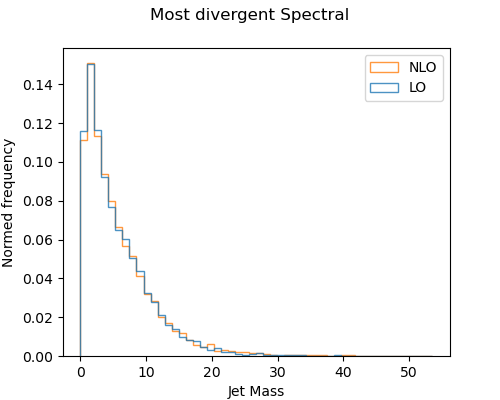
\includegraphics[width=\textwidth]{graphics/worst_spectral_histOnly.png}
%        \caption{The jet mass spectra of the Spectral algorithms that
%                 differed the most between LO and NLO datasets.
%                 This algorithm calculated affinities as
%                 \(a_{i,j} = \text{exp}\left((\delta \phi_{i, j}^2 + \delta y_{i, j}^2)/0.3\right)\).
%                 The Laplacian is symmetric and 
%                 as many eigenvector as can be found are used which are
%                 normalised as \(x_{i,\text{normed}} = x_i/\lambda_i^{1.8}\).
%                 There is no use of \(p_T\) and \(\stoppingdeltar{} = 1.3\).
%                 Little divergence can be seen.
%        }\label{fig:spectralircexample}
%    \end{minipage}
%    \begin{minipage}[c]{0.48\textwidth}
%        \includegraphics[width=\textwidth]{graphics/worst_iterativecone_histonly.png}
%        \caption{The jet mass spectra of the Iterative Cone algorithms that
%                 differed the most between LO and NLO datasets.
%                 This algorithm had a \(p_T\) exponent of \(1.\),
%                 (so the form of the \(p_T\) factor is between Cambridge-Aachen and KT),
%                 it used taxi-cab distances in physical space
%                 and \(\stoppingdeltar{} = 0.34\).
%                 Some divergence is seen, particularly at low mass.
%        }\label{fig:iterconeircexample}
%    \end{minipage}
\end{figure}    

%
%\begin{figure}[htp]
%    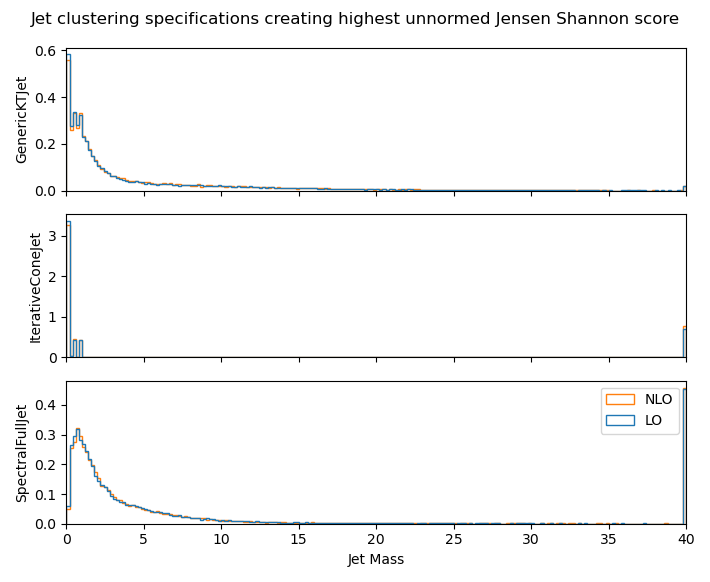
\includegraphics[width=1.\textwidth]{graphics/same_bin_size_worst_all_jets.png}
%    \caption{Same plots as previous, but with the same x-axis.
%        Last bin is overflow bin.
%    }
%\end{figure}    
%
However, this method of establishing IR safety only looks at one hyperparameter configuration and could be accused of cherry-picking.
As described in section~\ref{sec:IRmethod}, this can be systematically compared for many hyperparameter configurations by calculating a Jensen-Shannon
score for each LO and NLO pair of jet mass spectra.
If the Jensen-Shannon metric is low, then the two distributions are similar and appear IR safe.
To further clarify the result we include an algorithm known to be IR unsafe, the \itercone{} algorithm.
The spectral method produces Jensen-Shannon scores very similar to \genkt{} methods. Only the iterative cone one produces high Jensen-Shannon scores thus indicating significant changes between the LO and NLO spectra.
This can be seen in Fig.~\ref{fig:unnormedJS}. {\textcolor{red}{Is this plot done only using the Mass variable of the previous figure? If so, why this choice instead of, e.g., thrust, sphericity, oblataness or others?}\textcolor{blue}{H. fixed}}

\begin{figure}[htp]
    \begin{minipage}[c]{0.5\textwidth}
        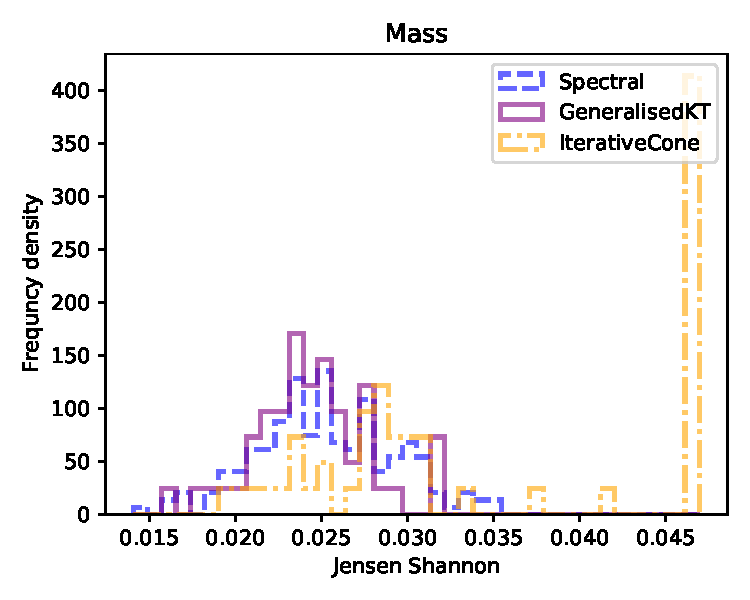
\includegraphics[width=1.\textwidth]{graphics/js_scores/Mass}
    \end{minipage}\hfill
    \begin{minipage}[c]{0.5\textwidth}
        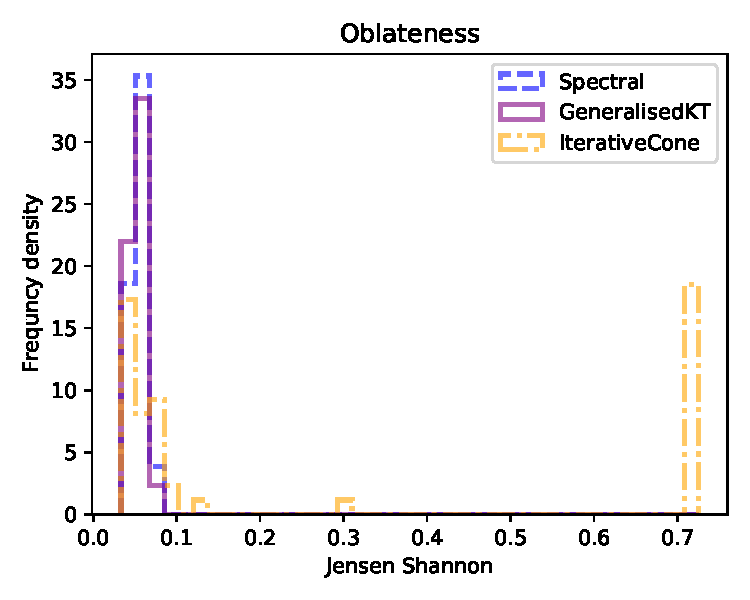
\includegraphics[width=1.\textwidth]{graphics/js_scores/oblateness}
    \end{minipage}
    \begin{minipage}[c]{0.5\textwidth}
        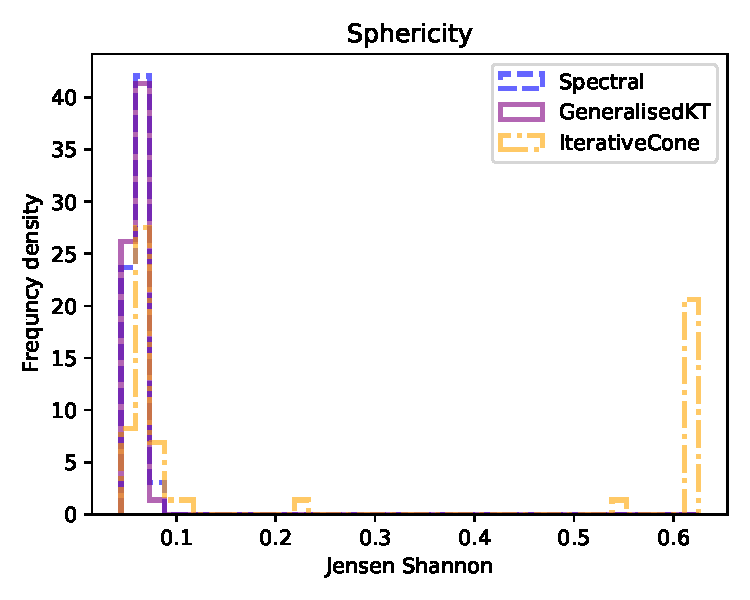
\includegraphics[width=1.\textwidth]{graphics/js_scores/sphericity}
    \end{minipage}\hfill
    \begin{minipage}[c]{0.5\textwidth}
        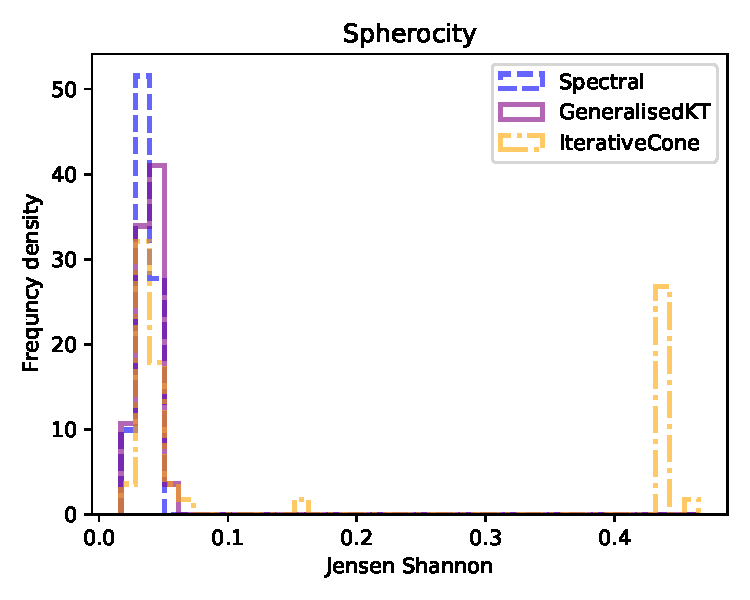
\includegraphics[width=1.\textwidth]{graphics/js_scores/spherocity}
    \end{minipage}
    \begin{minipage}[c]{0.5\textwidth}
        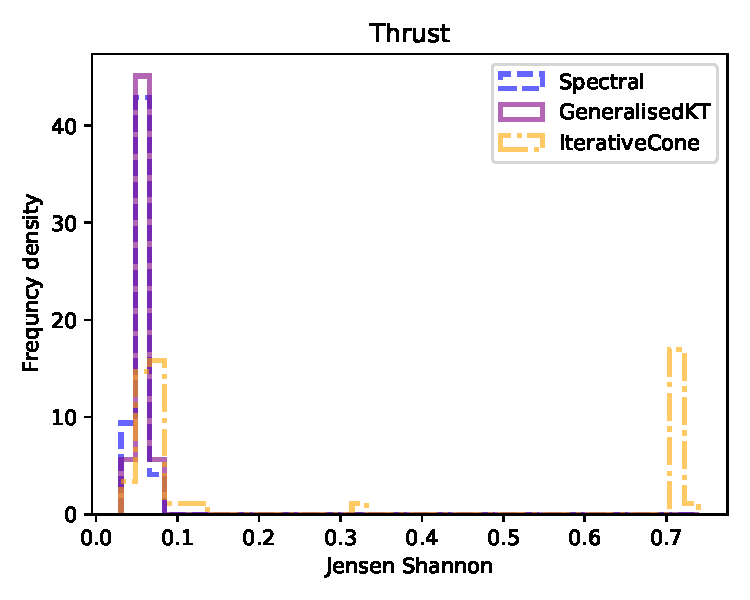
\includegraphics[width=1.\textwidth]{graphics/js_scores/thrust}
    \end{minipage}\hfill
    \begin{minipage}[c]{0.5\textwidth}
    \caption{
        Histograms evaluating IR safety from each jet shape variable.
        Each count is a  Jensen-Shannon score between a probability density of the
        jet shape variable from LO and NLO data.
        Counts at low values indicate insensitivity to IR differences between the LO and NLO data,
        thus IR safety.
     }\label{fig:unnormedJS}
    \end{minipage}
\end{figure}    

%This comparison is slightly complicated by the fact that we must use a completely different set of events,
%so if a clustering algorithm tends to produce more noisy mass spectra (on varied events), this
% will increase the gap between the LO and NLO datasets even if no IR sensitivity is present.
%Again, as described in section~\ref{sec:IRmethod}, the influence of this noise can be investigated.
%This can be seen in Fig.~\ref{fig:JensenShannon}. Here, 
%the subsampled Jensen-Shannon score is shown, again,  between a probability density of jet mass from LO and
%        NLO data, as described in section~\ref{sec:IRmethod}. Like in the previous figure, spectral clustering produces Jensen-Shannon scores similar to the \genkt{} approach. Likewise, only theiIterative cone produces high Jensen-Shannon scores, thus indicating significant changes
%        between the LO and NLO spectra. Being the results in  Figs.~\ref{fig:unnormedJS} and \ref{fig:JensenShannon} consistent with each other, this indicates  that the volume of data used to produce these
%        was sufficient to mitigate the effects of noise.

From  the last two figures it is clear that \spectral{} clustering  is IR safe, at least, as much as \genkt{} algorithms are.
This contrasts with the \itercone{} algorithm, for which the jet mass spectra at LO and NLO 
differ significantly for many configurations.
This is not unexpected, as the inputs to the \spectral{} clustering algorithm 
are the same as for the Cambridge-Aachen one, 
which is itself IR safe, and the iterative cone has been  proved to produce kinematic configurations which are IR unsafe \cite{Salam:2007xv} {\textcolor{red}{Please refer to some paper illustrating this (by Salam, Seymour, etc.)} \textcolor{blue}{H. done}} .
However, it is crucial to have such a verification in data, as we have done.

%\begin{figure}[htp]
%    \begin{minipage}[c]{0.6\textwidth}
%    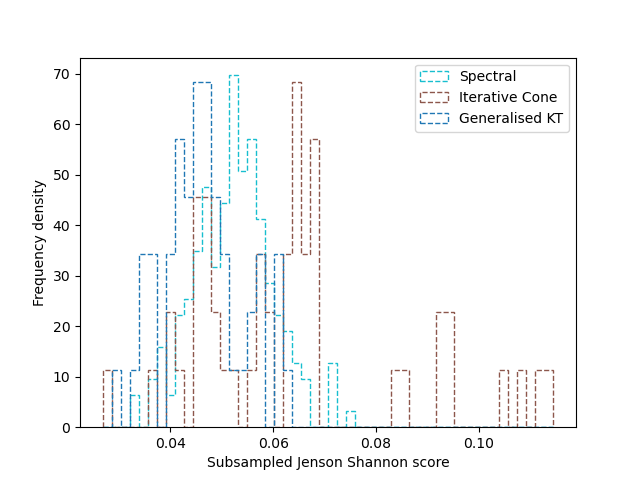
\includegraphics[width=1.\textwidth]{graphics/JensenShannon.png}
%    \end{minipage}\hfill
%    \begin{minipage}[c]{0.35\textwidth}
%    \caption{Same as Fig.~\ref{fig:unnormedJS} for the subsampled Jensen-Shannon score.
%    }\label{fig:JensenShannon}
%    \end{minipage}
%\end{figure}    

\subsection{Mass peak reconstruction}
In this section, the \antikt{} algorithm setups with jet radius \(\ktstoppingdeltar{} = 0.4\) and \(\ktstoppingdeltar{} = 0.8\)
are compared to the \spectral{} algorithm specified in section~\ref{sec:spectralmethodparam}.
The jets are tagged using MC truth.
Each of the \bthing{quarks} created by a signal particle (either a Higgs boson or a top (anti)quark)
tag the closest jet (by using the distance metric \(\sqrt{(y_\text{quark tag} - y_\text{jet})^2 + (\phi_\text{quark tag} - \phi_\text{jet})^2}\)
{\textcolor{red}{Do you really mean rapidity here or pseudorapidity? This needs to be clarified throughout as the two are not the same for massive objects} \textcolor{blue}{H. it is always rapidity, pesudorapidity is never used in this work, is Eqn~\ref{eqn:rapidity} alright?}})
provided that the separation between the jet and the quark is no greater than \(0.8\) according to the distance metric {\textcolor{red}{The sentence is unclear} \textcolor{blue}{improved?}}.
In the case of a \(W^\pm\) decay, whatever quarks decay from the \(W^\pm\), which may be light quarks or \bthing{quarks}, are used to tag jets in the same way.
From this point on, only jets tagged this way are considered {\textcolor{red}{What about light jets from $W^\pm$ decays?} \textcolor{blue}{Good point. Fixed.}}.


Firstly, jet multiplicities, that is number of reconstructed jets found per event, are given for both anti-$k_T$ and spectral clustering algorithms.
These can be seen for the first three datasets described in section~\ref{sec:particle_data} in Fig.~\ref{fig:multiplicity}. Herein, it
 is seen that \spectral{} clustering produces the best multiplicity (i.e., most events where 4 jets are found) for light Higgs events while for 
         the heavy Higgs and top MC samples  
        it creates a multiplicity closer to that of \antikt{} with \(\ktstoppingdeltar{} = 0.4\) 
        than \(\ktstoppingdeltar{} = 0.8\), the first of these being the best performer of the two. As a result of this study, we remark upon the adaptability of spectral clustering to the different final states without requiring adjusting its parameters, unlike the anti-$k_T$ one. The latter may seem to indicate that 0.4 is the best choice for all datasets, but this is in tension with the fact that different masses from different datasets do require the  anti-$k_T$ algorithm to be adjusted, as we shall now see. 



\begin{figure}[htp]
    \begin{center}
        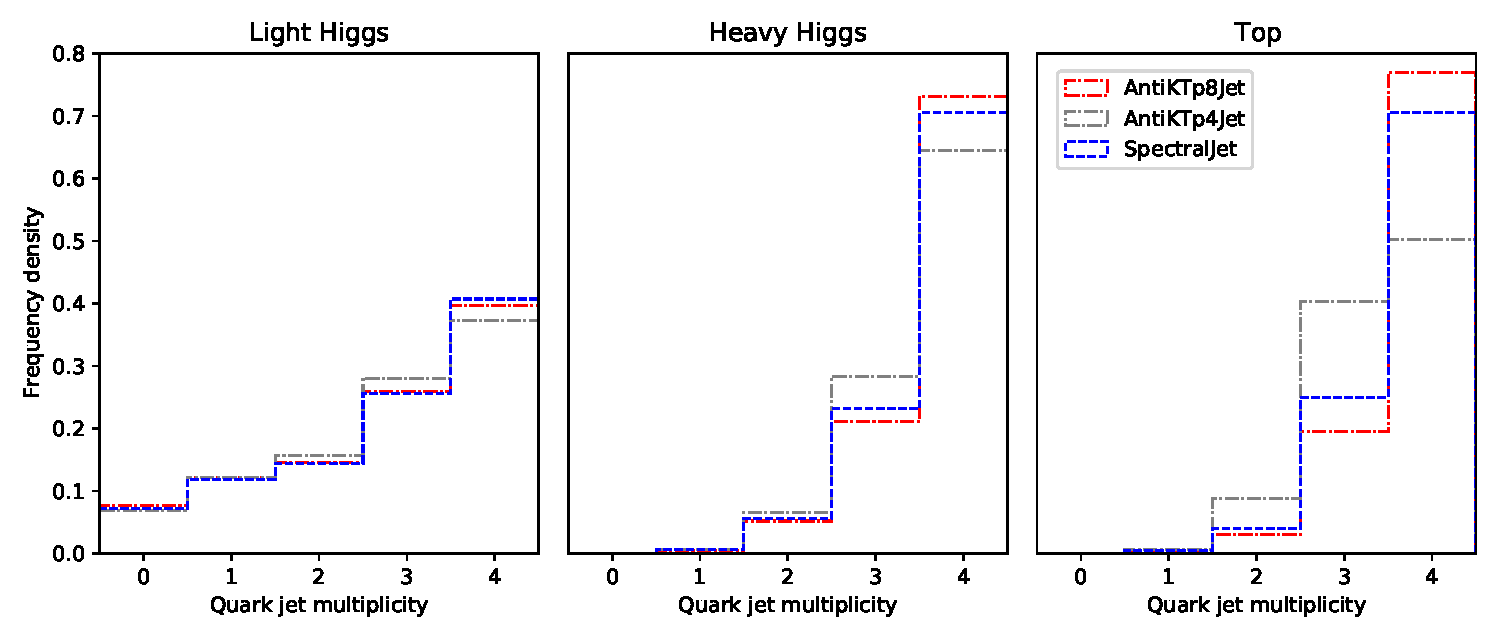
\includegraphics[width=1.0\textwidth]{graphics/multiplicity/multiplicity}
    \end{center}
    \caption{Jet multiplicities for the anti-$k_T$ (for two jet radius choices) and \spectral{} clustering algorithms on the light Higgs, heavy Higgs and top MC 
 samples. For all such datasets, the hard scattering produces  4 partons in the final  state, so maximising a multiplicity of 4 jets indicates good performance.   
    }\label{fig:multiplicity}
\end{figure}    



%As the data is simulated, it is possible to compare the performance of clustering algorithms to Monte Carlo truth.
%Each Higgs cascade event contains 4 \bthing{quarks} and for each of them it is possible to identify the particle into which they decayed, as a subset of the particles in the final state.
%Henceforth the detectable decay products of the \bthing{quark} will be called the descendants of the \bthing{quark}.
%For two reasons it is not possible for this clustering algorithm to gather all the descendants
%of each \bthing{quark} into one jet:
%firstly, not all the descendants make the \(p_T\) and \(\eta\) cuts, so some are discarded before clustering;
%secondly, the descendants of the \bthing{quarks} in an event are not mutually exclusive, due to interactions during hadronisation the quarks share descendants, and our clustering algorithm does produce exclusive clusters.
%
%Combining these factors with the \(p_T\) cuts, almost \(2/3\) of the objects could be reconstructed in theory.

%Knowing the parts of the final state that are descended from each \bthing{quark} creates a clear
%allocation of jets to quarks.
%For each quark, the jet that contains the greatest mass in descendent particles is tagged to represent that quark.

Mass peaks are constructed from the reconstructed jets as well as, for the top sample only, from the lepton and neutrino.
Again, the \antikt{} results  with \(\stoppingdeltar{}_{k_T} = 0.4\) and \(0.8\) are given for comparison.
In Fig.~\ref{fig:best_correct_h_allocation} three selections are plotted. Firstly, we show events where all 4 $b$-jets  
are plotted as total invariant mass of the event, thus reconstructing the mass of the SM Higgs boson.
Each event also contains two light Higgs states, though. These are differentiated by the mass of the particles (generating them) that pass the particle cuts,
as follows. The light Higgs boson reconstructed from the 2 $b$i-jet system with more mass visible to the detector is called the ``Light Higgs with stronger signal''
while the one reconstructed  with less mass visible in the detector is called the ``Light Higgs with weaker signal'' {\textcolor{red}{I do not really like this wording, I would suggest instead ``Most massive light Higgs'' and ``Lest massive light Higgs''} \textcolor{blue}{H., I don't think the mass of the higgs itself (the displacement offshell) has much influence on which higgs is which. It's a reflection of which higgs produces more decay products that pass the particle cuts, whcih reflect the detectors capacity to reconstruct particles according to pt and rapidity. What do you think of; ``Higgs producing stronger signal"/``Higgs producing weaker signal"?}}.
%Two jets are required to reconstruct a light Higgs.
The correct jets for each Higgs mass reconstruction are identified using MC truth,
so the correct pairings are always made. (If two such di-jet systems are not found the event is not included in the plots).
Altogether, it can be seen that spectral clustering forms the sharpest peaks and such peaks are all very close to the correct mass. In fact, its performance
is comparable to that of anti-$k_T$ with jet radius 0.8 and is clearly better than the 0.4 option. 


\begin{figure}[htp]
    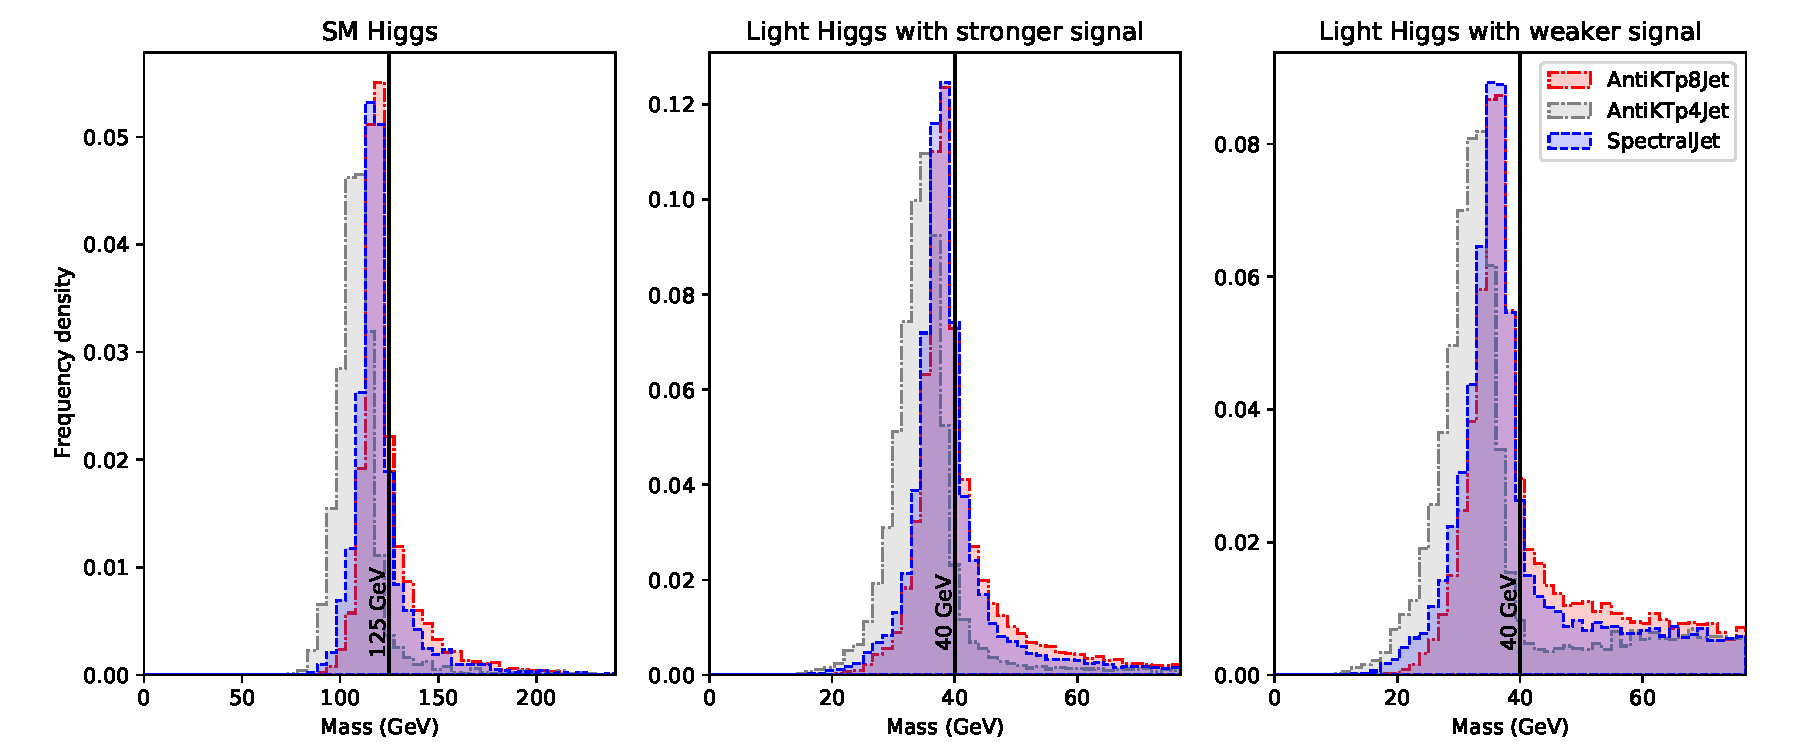
\includegraphics[width=1.\textwidth]{graphics/mass_peaks/light_long_correct_lines}
    \caption{Three mass selections are plotted for the light Higgs dataset. From left to right we show: the invariant mass of the 4 $b$-jet system, of the 2 $b$-jet system with heaviest invariant mass and of the 2 $b$-jet system with lightest invariant mass (as defined in the text).   Three jet clustering combinations are plotted as detailed in the legend.
        The spectral clustering algorithm is consistently the best performer in terms of the narrowest peaks being reconstructed and comparable to \antikt{} with \(\ktstoppingdeltar{} = 0.8\) in terms of its shift from the true Higgs mass values, with \antikt{} with \(\ktstoppingdeltar{} = 0.4\) always being the outlier. 
{\textcolor{red}{Higgs should be capitalised as Higgs in the top titles, though, see my remark in the body for the actual names} \textcolor{blue}{H. done}}
    }\label{fig:best_correct_h_allocation}
\end{figure}    

In 
Fig.~\ref{fig:heavy_correct_mass_peaks} the exercise is repeated for the heavy Higgs dataset.
All the parameters of \spectral{} clustering are the same as in the light Higgs MC sample yet we note that 
its performance is still excellent, with very sharp peaks at the correct masses, although the three clustering algorithms are overall much closer in performance.
However, recall that, in Fig.~\ref{fig:multiplicity},
it was seen that spectral clustering achieved better multiplicity than \antikt{} with \(\ktstoppingdeltar{} = 0.8\) on this dataset. Furthermore, 
while the multiplicity of \antikt{} with \(\ktstoppingdeltar{} = 0.4\) is a little better, the location of all Higgs mass peaks for anti-$k_T$ with 
\(\ktstoppingdeltar = 0.4\) is slightly worse. So, we are again driven to conclude that spectral clustering is probably the best performer overall with the added benefit of not requiring any adjustment of its parameters to achieve it. 

\begin{figure}[htp]
    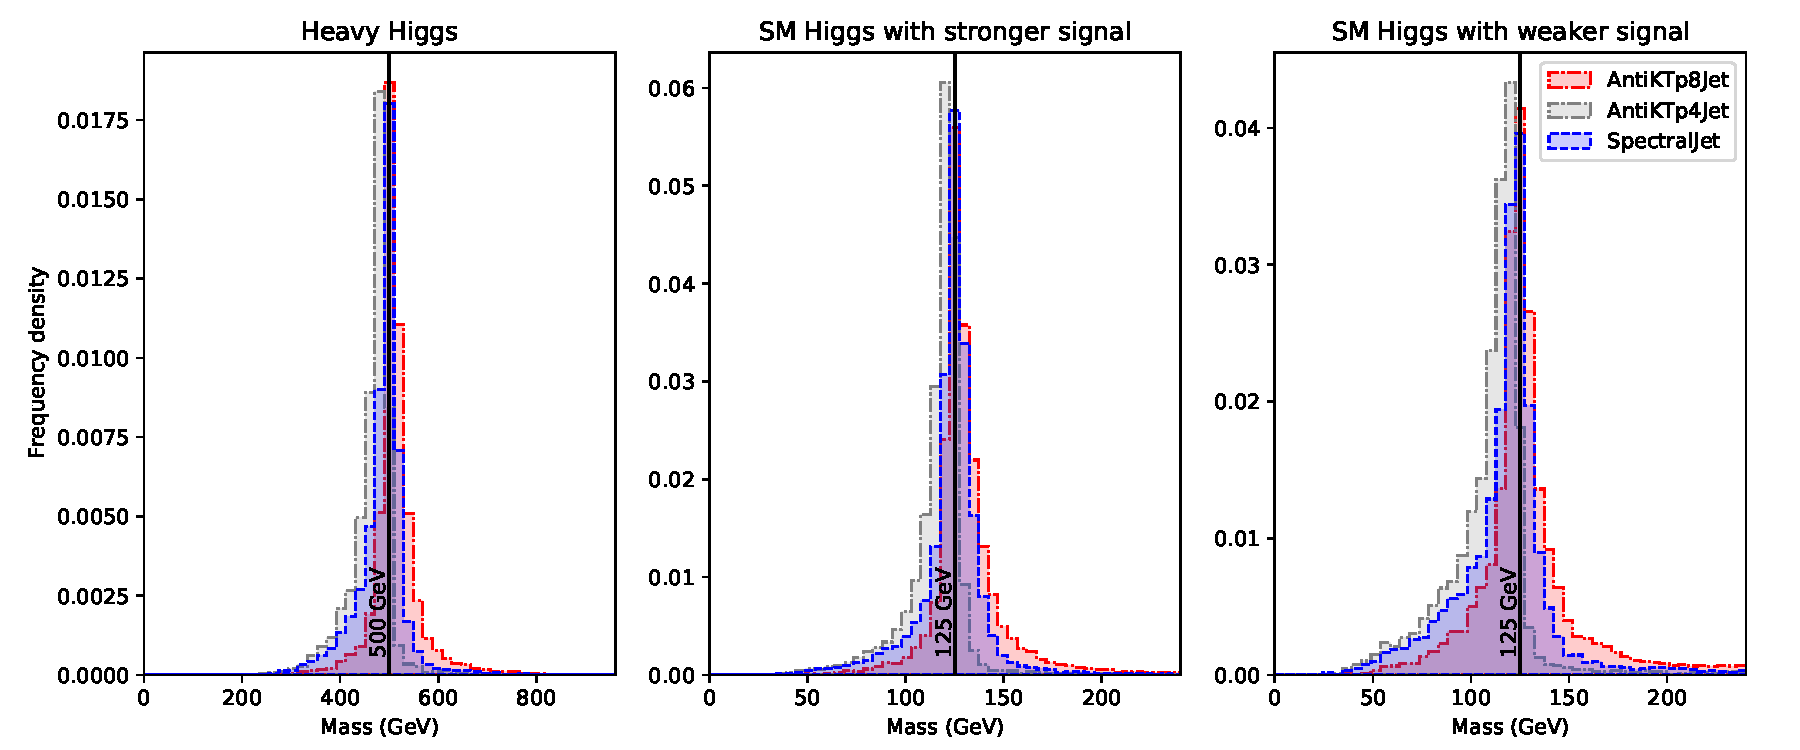
\includegraphics[width=1.\textwidth]{graphics/mass_peaks/heavy_long_correct_lines}
    \caption{Same as Fig.~\ref{fig:best_correct_h_allocation} for the heavy Higgs dataset. Here, the performance of the spectral clustering and anti-$k_T$ (with both 0.4 and 0.8 as jet radiuses) clustering is much closer to each other. 
}\label{fig:heavy_correct_mass_peaks}
\end{figure}    


\begin{figure}[htp]
    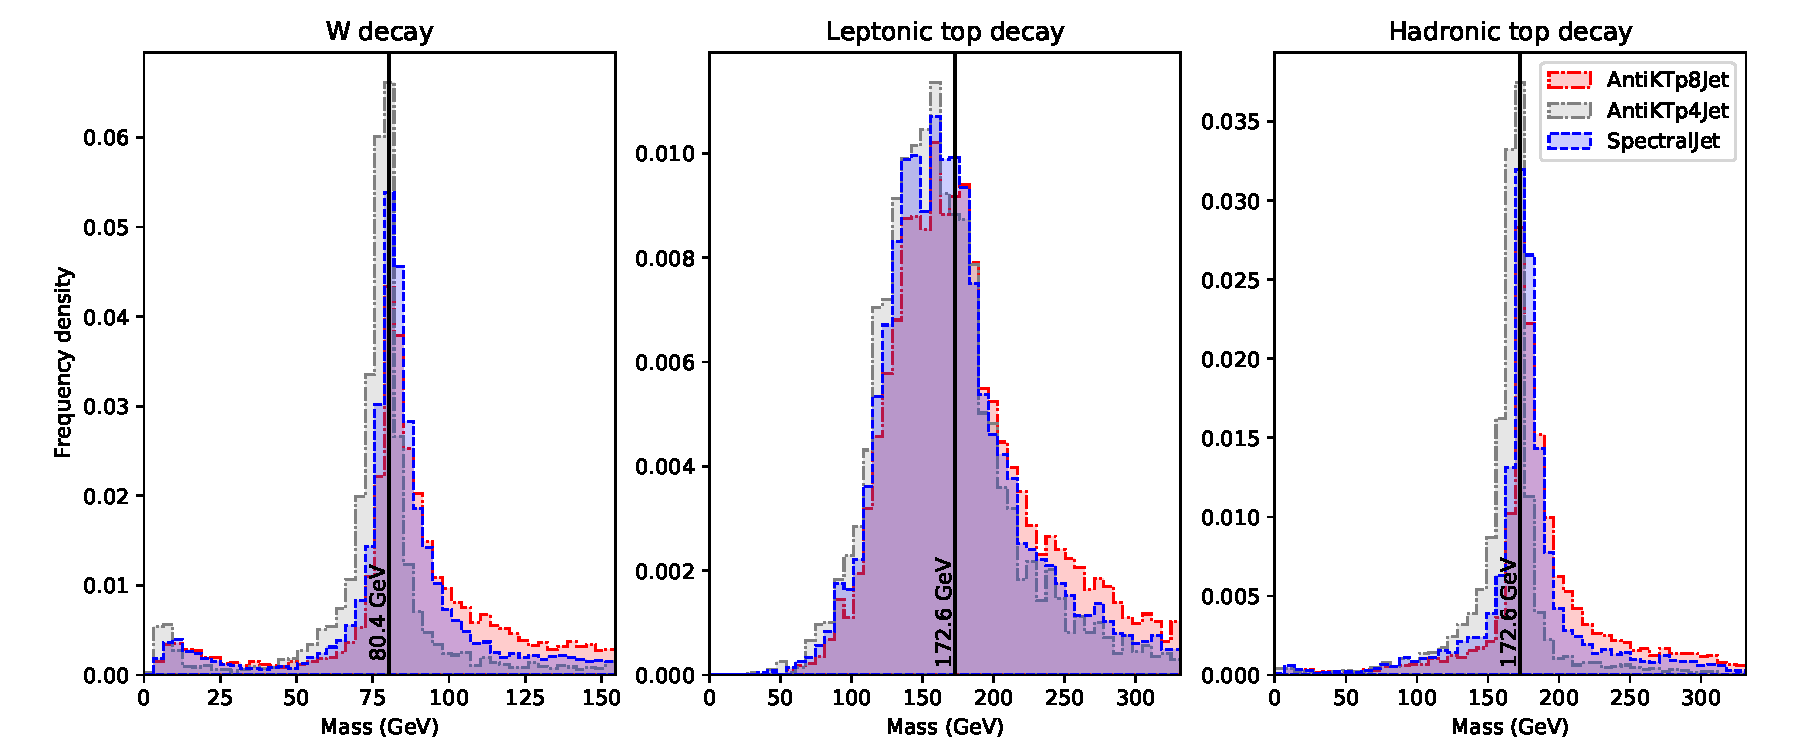
\includegraphics[width=1.\textwidth]{graphics/mass_peaks/top_long_correct_lines}
    \caption{Three mass selections are plotted for the top dataset. From left to right we show: the invariant mass of the light jet system, of the reconstructed leptonic $W^\pm$ (as  described in the text) combined with a $b$-jet and of the hadronic $W^\pm$ combined with the other $b$-jet. Three jet clustering combinations are plotted as detailed in the legend.
The spectral clustering algorithm  consistently outperforms the  anti-$k_T$ one with jet radius 0.8 and is slightly worse than the anti-$k_T$ one with jet radius 0.4, but only in tems of sharpness, not location.
    }\label{fig:top_correct_mass_peaks}
\end{figure}    

Finally, in Fig.~\ref{fig:top_correct_mass_peaks}, the $W^\pm$ and $t$ mass peaks for semileptonic $t\bar t$ decays are shown.
Three mass reconstructions are given.
Firstly, the hadronic \(W\) is reconstructed from the jets that come from the quarks it decayed to.
Correct decisions about which quarks correspond to which particle in the hard process are made by using information in the Monte Carlo,
this is to prevent any mismatching from causing additional complication in evaluating the performance of the clustering.
To tag a jet with a quark a distance measure \(\sqrt{(y_\text{quark tag} - y_\text{jet})^2 + (\phi_\text{quark tag} - \phi_\text{jet})^2}\)
is used, and if the distance from the quark to the closest jet is less than \(0.8\) that jet is tagged by that quark.
The \(W\) will always decay to a pair of quarks, but both these quarks may be captured in one jet or separate jets.
{\textcolor{red}{This sentence did not make sense at all} \textcolor{blue}{H. is this better?}}.
If either of the these quarks are too far away from the closest jet to tag it,
that is \(\sqrt{(y_\text{quark tag} - y_\text{jet})^2 + (\phi_\text{quark tag} - \phi_\text{jet})^2} > 0.8\),
then it is not associated with any jet and the hadronic \(W\) is not reconstructed.
{\textcolor{red}{This sentence did not make sense either} \textcolor{blue}{H. is this better?}}.
The mass of the hadronic top is then reconstructed in events where the hadronic \(W\) could be reconstructed and the \bthing{jet}
from the hadronic top is also found. {\textcolor{red}{By MC truth or you pick the $b$ that gives the best $m_t$? Please clarify} \textcolor{blue}{H., always MC truth, I will clarify this at the start of the passage.}}.
The leptonic top is then reconstructed in events where \bthing{jet} from the top is combined with the reconstructed $W^\pm$ which as decayed leptonically
{\textcolor{red}{By MC truth or pick the $b$ that gives the best $m_t$? Please clarify}\textcolor{blue}{H. ditto}}.
The leptonic reconstruction of the $W^\pm$ uses the momentum of the electron $p_\ell$, the missing transverse momentum $p_T^{\rm miss}$ (identified with that of the neutrino)
and the longitudinal neutrino momentum ($p_L^\nu$, which is unknown) in a quadratic equation, $(p_\ell+p_T^{\rm miss}+p_L^\nu)^2=m_W^2$, of which only the real solutions are plotted.  In this case, it can be seen that \spectral{} clustering is adapting to jets of a different radius. In fact, 
while before its behaviour had mostly resembled anti-$k_T$ with \(\ktstoppingdeltar{} = 0.8\), 
it has now moved closer to the case with \(\ktstoppingdeltar{} = 0.4\).
(Semileptonic top events would typically be processed using anti-$k_T$ with \(\ktstoppingdeltar{} = 0.4\).)
The peaks of \spectral{} clustering are not quite as narrow as those from anti-$k_T$ with \(\ktstoppingdeltar{} = 0.4\),
but they improve on \(\ktstoppingdeltar{} = 0.8\) and their  location is substantially correct.

%\begin{figure}[htp]
%    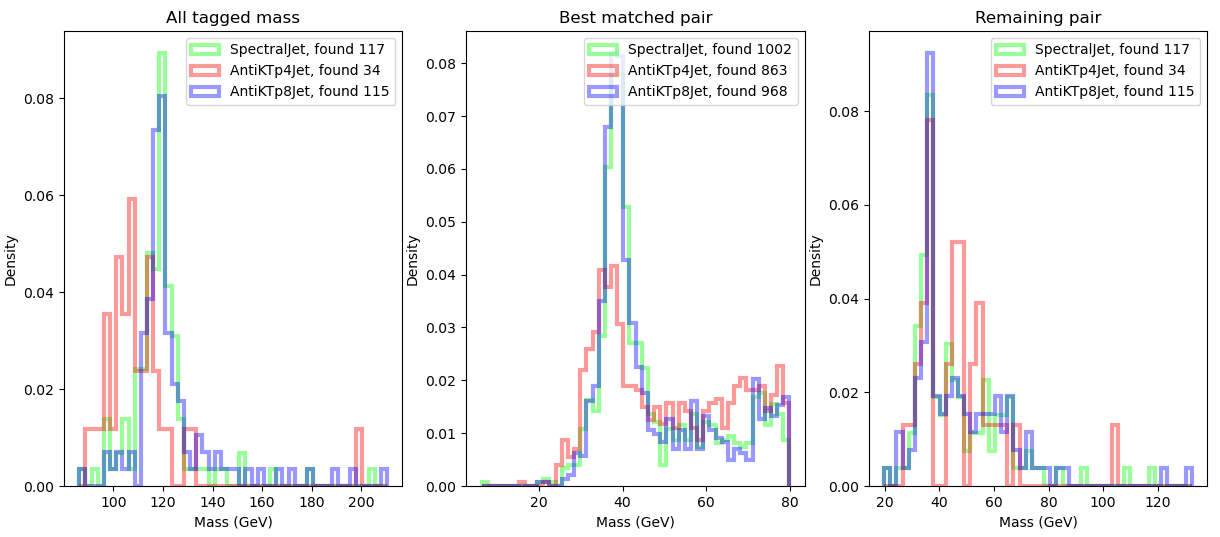
\includegraphics[width=1.\textwidth]{graphics/show2_40.png}
%    \caption{Mass peaks for the light Higgs cascade;
%    \(p^+ p^+ \rightarrow H_{125\text{GeV}} \rightarrow h_{40\text{GeV}} h_{40\text{GeV}} \rightarrow \beau \bbar \beau \bbar\).
%        Jets are required to have at least 2 particles and \(15\) GeV \(p_T\).
%        The left hand peak is the mass of all jets in events where 4 jets are reconstructed.
%        The central plot is the mass of the dijet pair closest to \(40\) GeV,
%        the right hand plot is the remaining dijet pair.
%    }
%\end{figure}    
%
%\begin{figure}[htp]
%    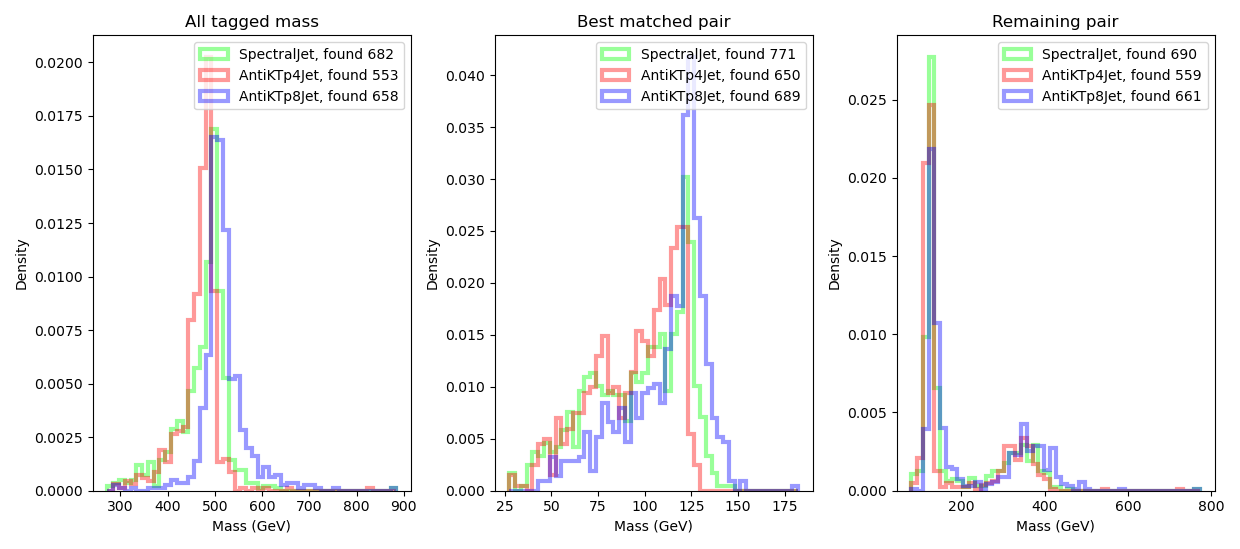
\includegraphics[width=1.\textwidth]{graphics/show2_125.png}
%    \caption{Mass peaks for the heavy Higgs cascade,
%    \(p^+ p^+ \rightarrow H_{500\text{GeV}} \rightarrow h_{120\text{GeV}} h_{120\text{GeV}} \rightarrow \beau \bbar \beau \bbar\).
%        Jets are required to have at least 2 particles and \(30\) GeV \(p_T\).
%        The left hand peak is the mass of all jets in events where 4 jets are reconstructed.
%        The central plot is the mass of the dijet pair closest to \(125\) GeV,
%        the right hand plot is the remaining dijet pair.
%    }
%\end{figure}    



%There are also some values that can be given to compare these two jets;
%\begin{enumerate}
%    \item Quality fraction~\cite{JetQuality2008}. A window on the reconstructed masses,
%        size proportional to the root of mass of the object to be reconstructed,
%        across the data. The total number of generated objects (in this dataset 2000)
%        is divided by the maximum number of reconstructed objects in the window,
%        and this is the quality width.
%        
%        \[\text{\antikt{} (\(\stoppingdeltar{} = 0.8\)) Quality Fraction} = 1.33\text{GeV}\]
%        \[\text{Spectral Quality Fraction} = 1.33\text{GeV}\]
%    \item Quality width~\cite{JetQuality2008}. A required fraction of the generated objects,
%        in this case \(0.15\) is selected.
%        The smallest mass window that can capture this fraction is determined.
%        
%        \[\text{\antikt{} (\(\stoppingdeltar{} = 0.8\)) Quality Width} = 0.00141\text{GeV}\]
%        \[\text{Spectral Quality Width} = 0.000129\text{GeV}\]
%    \item Signal mass lost. The mass of the particles descendent from the light Higgs
%        that are visible on the barrel is compared to the mass of the subset of those
%        particles that was found in the jet. The higher the number the more
%        signal particles are missing from the jet.
%        \[\text{\antikt{} (\(\stoppingdeltar{} = 0.8\)) Signal mass lost} = 1.80\text{GeV}\]
%        \[\text{Spectral Signal mass lost} = 2.17\text{GeV}\]
%    \item Background contamination. The mass of all the background objects,
%        either from the wrong Higgs or from gluons, found in jets.
%        The higher the number the more the jets are tending to include too many particles.
%        \[\text{\antikt{} (\(\stoppingdeltar{} = 0.8\)) Background contamination} = 1.92\text{GeV}\]
%        \[\text{Spectral Background contamination} = 1.56\text{GeV}\]
%\end{enumerate}
%

    \FloatBarrier
    \section{Conclusions}
Spectral clustering offers a promising new jet formation method.
It is a transparent mechanism with no black box element.
All intermediate steps are interpretable.
It satisfies the need for IRC safety and creates jets with the expected kinematics.

While it has many hyperparameters, then do not appear to be as finely tuned as those of \genkt{}.
This can be seen both in parameter scans, and its adaptability to various datasets.

The adaptability between datasets is remarkable,
a \spectral{} parameter choice tuned on a light higgs cascade
gave excellent performance on both a heavy higgs cascade and a top decay.
On the light higgs cascade \spectral{} gives the correct mass peak,
a narrow mass peak and the highest multiplicity.
This would not be surprising as it was tuned for that dataset.
On the heavy higgs dataset only \antikt{} \(\ktstoppingdeltar{} = 0.8\) 
and \spectral{} give correct mass peaks, and \spectral{} offers considerably higher multiplicities.
This demonstrates that the performance is not dependent on fine tuning and the algorithm is adaptable.

Finally, \spectral{} was applied to a dataset for which the ideal jet radius differed.
Its equivalent parameter \(\sigma_v\) was not allowed to vary to account for this,
instead it was applied again with no parameter changes.
The algorithm again proved to be adaptable and modified its behaviour to follow that of \(\ktstoppingdeltar{} = 0.4\)
without interference.

This is a novel and promising approach to jet formation. 
Initial development already demonstrates flexibility and excellent performance.


    \FloatBarrier
    \section{Acknowledgements}
We thank A. Chakraborty, 
G. Cerro, 
J. Chaplais, 
S. Jain and 
E. Olaiya fur insightful discussions. HAD-H thanks
G.P. Salam for useful advice. 
HAD-H, BF, SM and CHS-T are supported in  in part through the NExT Institute.
SM is also supported by the STFC Consolidated
Grant No. ST/L000296/1. BF is funded by the DISCnet \& SEPnet scholarship schemes.
We finally 
acknowledge the use of the IRIDIS High Performance Computing Facility, and associated
support services, at the University of Southampton, in the completion of this work.
{\textcolor{red}{Others}}

\printbibliography
\end{document}
